\chapter{Reinforcement learning}


\section{Definitions}

\Acl{rl} (\acs{rl}) methods aim to maximize future reward by mapping the possible states of an environment into actions.

\begin{description}
    \item[Optimal decision making] \marginnote{Optimal decision making}
        Aims to maximize rewards and minimize punishments.

        \begin{remark}
            This is a difficult task as the outcome might be delayed or depend on a series of actions.
            
            \begin{descriptionlist}
                \item[Credit assignment problem]
                    Determine how the various factors involved in making a decision contributed to the success or failure of it.
            \end{descriptionlist}
        \end{remark}
\end{description}

\begin{remark}
    Multiple competing sub-systems contribute to learning and controlling behavior in animals.

    \begin{example}[Freud's theory of the mind structure]
        The mind is composed of three structures:
        \begin{descriptionlist}
            \item[Ego]
                Mainly works at the conscious level.
                Rational part of the mind that mediates \textit{id} impulses and \textit{superego} inhibitions.

            \item[Superego] 
                Mainly works at the preconscious level.
                Includes one's ideals and morals. Strives for perfection.

            \item[Id] 
                Mainly works at the unconscious level.
                Irrational part of the mind based on basic impulses that seek immediate gratification.
        \end{descriptionlist}
    \end{example}
\end{remark}


\subsection{Learning}

\begin{description}
    \item[Learning] \marginnote{Learning}
        Lasting change in response or behavior originated from experience.

    \item[Non-associative learning] \marginnote{Non-associative learning}
        Change in response or behavior caused by learning the properties of a single stimulus.
        It can result in:
        \begin{descriptionlist}
            \item[Habituation] 
                A decrease in response to a stimulus that is presented repeatedly.
                \begin{example}
                    The first explosion of a firework causes a strong response but the responses to the following ones are much weaker.
                \end{example}

            \item[Sensitization] 
                An increase in response to a stimulus that is presented repeatedly.
                \begin{example}
                    When the skin itches, one will start scratching it.
                \end{example}
        \end{descriptionlist}

    \item[Associative learning] \marginnote{Associative learning}
        Change in response or behavior caused by learning an association of two or more stimuli/events.

        \begin{descriptionlist}
            \item[\Acl{rl}] \marginnote{\Acl{rl}}
                Learn an association between a neutral stimulus (something the body considers irrelevant) and 
                a reinforcer (something the body considers relevant).

                \begin{description}
                    \item[Primary reinforcer] \marginnote{Primary reinforcer}
                        Positive or negative stimulus that is biologically relevant and elicits a response.
                        \begin{example}
                            Food, pain, social interactions, \dots
                        \end{example}

                    \item[Secondary reinforcer] \marginnote{Secondary reinforcer}
                        Positive or negative stimulus that became relevant following associative learning.
                        It elicits a response which usually enables a primary reinforcer.
                \end{description}
        \end{descriptionlist}
\end{description}


\subsection{Learning systems}

\begin{description}
    \item[Pavlovian/classical system] \marginnote{Pavlovian system}
        Form of prediction learning.
        Learns to predict biologically relevant stimuli to trigger an appropriate response (stimulus-outcome associations).

    \item[Instrumental system] \marginnote{Instrumental system}
        Form of control learning to learn action-outcome associations.
        It includes:
        \begin{descriptionlist}
            \item[Habitual system] \marginnote{Habitual system}
                Learn to repeat previously successful actions.
            \item[Goal-directed system] \marginnote{Goal-directed system}
                Evaluate actions based on the prior knowledge of their consequences.
        \end{descriptionlist}
\end{description}

\begin{remark}
    Pavlovian and instrumental systems are not independent.
    By predicting which situations are positive, one can act to reach them through its actions.

    \begin{figure}[H]
        \centering
        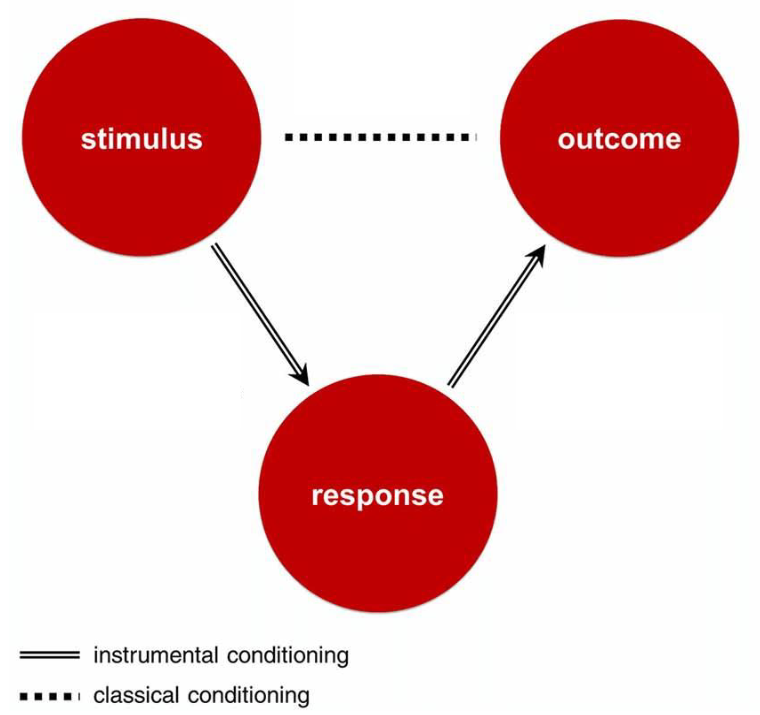
\includegraphics[width=0.35\linewidth]{./img/learning_systems.png}
        \caption{Learning systems relationship}
    \end{figure}
\end{remark}



\section{Learning at the neuronal level}

\begin{description}
    \item[Hebbian plasticity] \marginnote{Hebbian plasticity}
        Learning and experience change the connections of a neural system.

    \item[Short-term change] \marginnote{Short-term neuronal change}
        Functional physiological change that modifies the effectiveness of existing synaptic connections (i.e. amount of neurotransmitters).
        Lasts from seconds up to hours.

    \item[Long-term change] \marginnote{Long-term neuronal change}
        Structural change that leads to anatomical alterations such as pruning or growth of synapses.
        Lasts days and can cause further short-term changes.
\end{description}

\begin{remark}
    Neuronal changes follow a "use it or lose it" policy:
    only useful changes will last.
\end{remark}

\begin{example}[Phantom limb pain]
    In amputees, the area of the brain responsible for the missing part of the body is overrun by the neighboring sections.
    In the case of an arm, the area responsible for the face might "conquer" what once was the area of the arm.
\end{example}



\section{Pavlovian learning}
\marginnote{Pavlovian learning}

Form of prediction learning that aims to learn stimulus-outcome associations:
\begin{itemize}
    \item When a reinforcer is likely to occur.
    \item Which stimuli tend to precede a reinforcer.
\end{itemize}
This allows the animal to emit a response in anticipation of a reinforcer.

Pavlovian learning works as follows:\\
\begin{minipage}{0.58\linewidth}
    \begin{enumerate}[label=\alph*.]
        \item A stimulus that has no meaning to the animal will result in \ac{nr}.
        \item An \ac{us} (i.e. a reinforcer) generates an \ac{ur}.
        \item Learning happens when a reinforcer is paired with a non-relevant stimulus.
        \item The learned \ac{cs} generates a \ac{cr}.
    \end{enumerate}
\end{minipage}
\begin{minipage}{0.4\linewidth}
    \raggedleft
    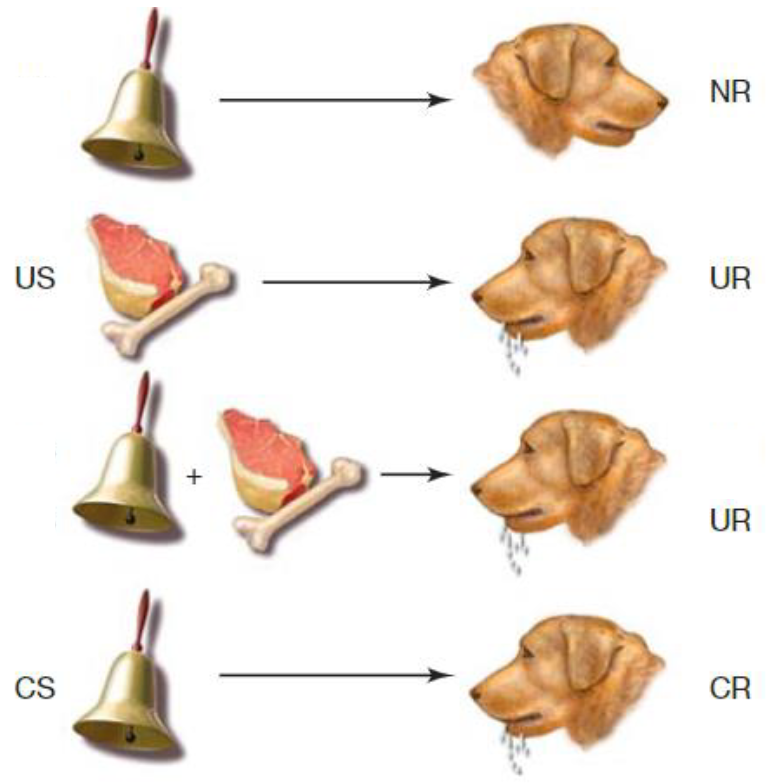
\includegraphics[width=0.9\linewidth]{./img/pavlovian_example.png}
\end{minipage}\\

An outcome can be:
\begin{descriptionlist}
    \item[Appetitive] Something considered positive.
    \item[Aversive] Something considered negative.
\end{descriptionlist}

The learned \acl{cr} can be:
\begin{descriptionlist}
    \item[Behavioral] Associated to the startle response (i.e. reflex in response to a sudden stimulus).
    \item[Physiological] Associated to the autonomic system.
    \item[Change in subjective response] 
\end{descriptionlist}

\begin{remark}
    Pavlovian learning has its foundations in behaviorism: the brain starts as a blank slate and only observable behaviors can be studied.
\end{remark}


\subsection{Types of reinforcement}

There are two types of learning:
\begin{descriptionlist}
    \item[Continuous reinforcement] \marginnote{Continuous reinforcement}
        The \acl{cs} is reinforced every time the \acl{us} occurs.
        \begin{remark}
            More effective to teach a new association.
        \end{remark}

    \item[Partial reinforcement] \marginnote{Partial reinforcement}
        The \acl{cs} is not always reinforced.
        \begin{remark}
            Learning is slower but the \acl{cr} is more resistant to extinction.
        \end{remark}
\end{descriptionlist}


\subsection{Learning flexibility}

\begin{description}
    \item[Acquisition] \marginnote{Acquisition}
        The probability of occurrence of a \acl{cr} increases if the \acl{cs} is presented with the \acl{us}.
        
    \item[Extinction] \marginnote{Extinction}
        The probability of occurrence of a \acl{cr} decreases if the \acl{cs} is presented alone.
\end{description}

\begin{remark}
    Extinction does not imply forgetting.
    After an association between \ac{cs} and \ac{us} is made, 
    extinction consists of creating a second association with inhibitory effects that overrides the existing association.

    The extinct association can return in the future
    (this is more evident when the context is the same as the acquisition phase).
\end{remark}

\begin{figure}[H]
    \centering
    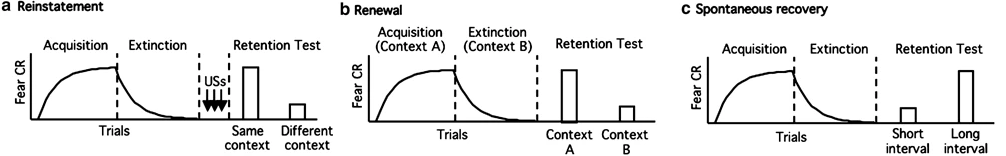
\includegraphics[width=0.95\linewidth]{./img/pavlovian_extinction.png}
    \caption{Example of acquisition, extinction, and \ac{cr} return}
\end{figure}

\begin{description}
    \item[Generalization] \marginnote{Generalization} 
        A new stimulus that is similar to a learned \acl{cs} can elicit a \acl{cr}.
\end{description}

\begin{example}[Aplysia Californica] \phantom{}\\
    \begin{minipage}{0.8\linewidth}
        \begin{enumerate}
            \item Before conditioning, a stimulus to the siphon of an aplysia californica results in a weak withdrawal of the gill.
            \item During conditioning, a stimulus to the siphon is paired with a shock to the tail which results in a large withdrawal of the gill.
            \item After conditioning, a stimulus to the siphon alone results in a large withdrawal response.
        \end{enumerate}
    \end{minipage}
    \begin{minipage}{0.18\linewidth}
        \centering
        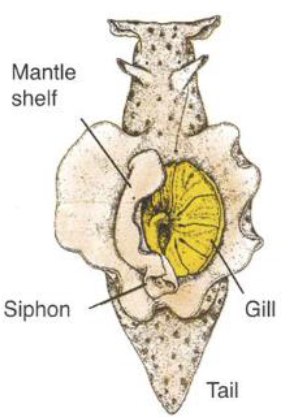
\includegraphics[width=\linewidth]{./img/aplysia.png}
    \end{minipage}

    \begin{figure}[H]
        \centering
        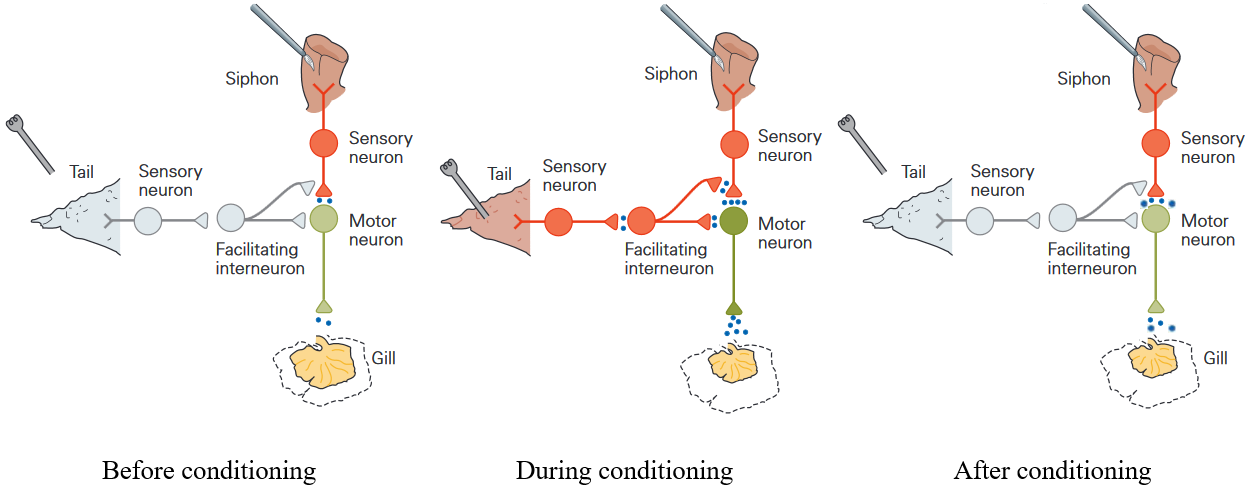
\includegraphics[width=0.85\linewidth]{./img/gill_pavlovian.png}
        \caption{Conditioning process}
    \end{figure}

    The learned response lasts for days.
    It can be observed that without training, the response disappears faster.

    \begin{figure}[H]
        \centering
        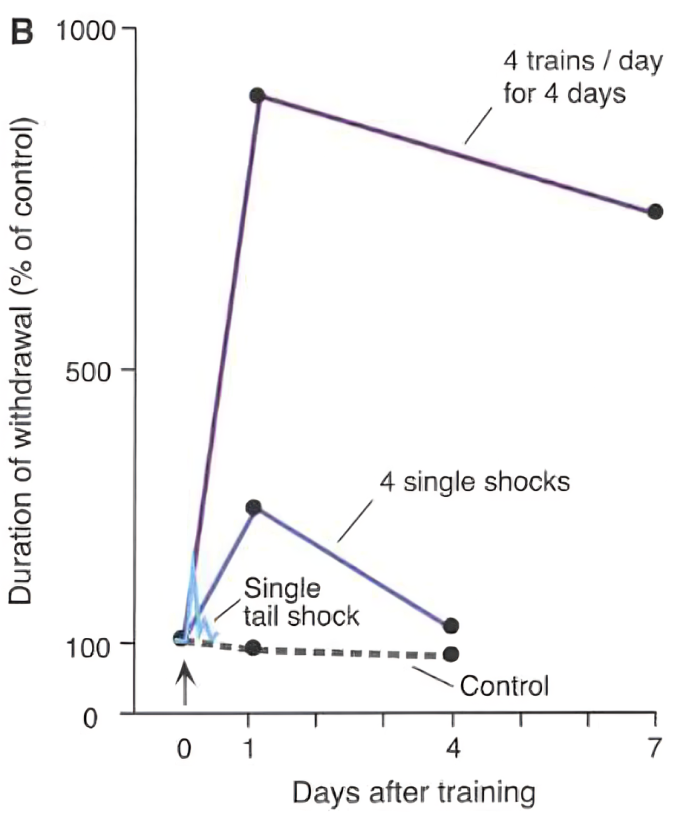
\includegraphics[width=0.35\linewidth]{./img/gill_pavlovian_graph.png}
        \caption{Withdrawal response decay}
    \end{figure}
\end{example}

\begin{remark} \marginnote{Amygdala in Pavlovian learning}
    In mammals, aversive Pavlovian conditioning involves the amygdala.
    The \ac{cs} and \ac{us} are relayed from the thalamus and the cerebral cortex to the amygdala, 
    which in turn connects to various motor responses such as:
    \begin{descriptionlist}
        \item[Central gray region (CG)] Controls the freezing behavior.
        \item[Lateral hypothalamus (LH)] Controls autonomic responses.
        \item[Paraventricular hypothalamus (PVN)] Controls stress hormones.
    \end{descriptionlist}

    \begin{figure}[H]
        \centering
        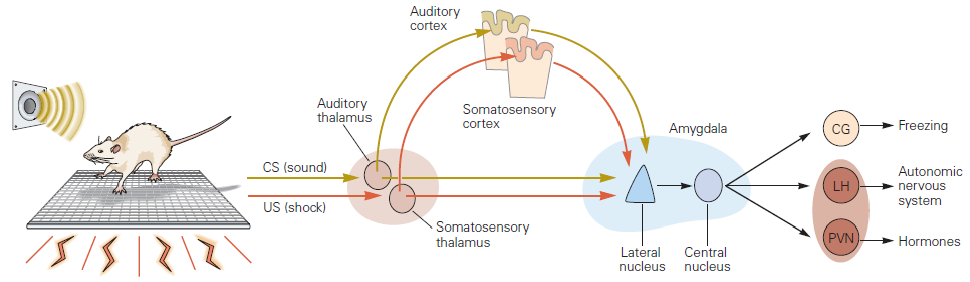
\includegraphics[width=0.9\linewidth]{./img/amygdala_pavlovian.png}
        \caption{Neural circuits during aversive conditioning}
    \end{figure}
\end{remark}



\section{Instrumental learning}
\marginnote{Instrumental learning}

Form of control learning that aims to learn action-outcome associations:
\begin{itemize}
    \item When a reinforcer is likely to occur.
    \item Which actions bring to those reinforcers.
\end{itemize}
This allows the animal to act in anticipation of a reinforcer.

Depending on the outcome, the effect varies:
\begin{descriptionlist}
    \item[Positive reinforcement] \marginnote{Positive reinforcement}
        Delivering an appetitive outcome to an action increases the probability of emitting it.

    \item[Positive punishment] \marginnote{Positive punishment}
        Delivering an aversive outcome to an action decreases the probability of emitting it.
    
    \item[Negative reinforcement] \marginnote{Negative reinforcement}
        Omitting an aversive outcome to an action increases the probability of emitting it.
    
    \item[Negative punishment] \marginnote{Negative punishment}
        Omitting an appetitive outcome to an action decreases the probability of emitting it.
\end{descriptionlist}

\begin{table}[H]
    \centering
    \begin{tabular}{r|cc}
        \toprule
                            & \textbf{Delivery}                         & \textbf{Omission} \\
        \midrule
        \textbf{Appetitive} & Positive reinforcement (\texttt{+prob})   & Negative punishment (\texttt{-prob}) \\
        \textbf{Aversive}   & Positive punishment (\texttt{-prob})      & Negative reinforcement (\texttt{+prob}) \\
        \bottomrule
    \end{tabular}
    \caption{Summary of the possible effects}
\end{table}


\subsection{Types of schedule}

There are two types of learning:
\begin{descriptionlist}
    \item[Continuous schedule] \marginnote{Continuous schedule}
        The desired action is followed by the outcome every time.
        \begin{remark}
            More effective to teach a new association.
        \end{remark}

    \item[Partial schedule] \marginnote{Partial schedule}
        The desired action is not always followed by the outcome.
        \begin{remark}
            Learning is slower but the response is more resistant to extinction.
        \end{remark}

        There are four types of partial schedules:
        \begin{descriptionlist}
            \item[Fixed-ratio] 
                Outcome available after a specific number of responses.

                This results in a high and steady rate of response, with a brief pause after the outcome is delivered.


            \item[Variable-ratio] 
                Outcome available after an unpredictable number of responses.

                This results in a high and steady rate of response.


            \item[Fixed-interval] 
                Outcome available after a specific interval of time.

                This results in a high rate of response near the end of the interval and a slowdown after the outcome is delivered.


            \item[Variable-interval] 
                Outcome available after an unpredictable interval of time.

                This results in a slow and steady rate of response.
        \end{descriptionlist}
\end{descriptionlist}

\begin{example}[Aplysia Californica]
    An Aplysia Californica will withdraw its gill upon stimulating the siphon.
    \begin{itemize}
        \item Repeated mild stimulations will induce a habituation of the reflex.
        \item Repeated intense stimulations will induce a sensitization of the reflex.
    \end{itemize}

    \begin{figure}[H]
        \centering
        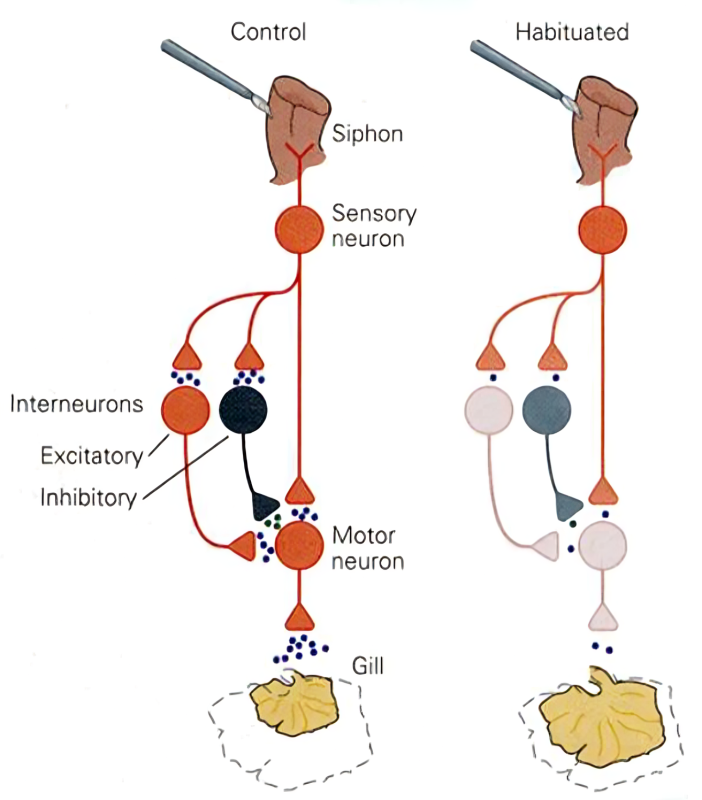
\includegraphics[width=0.4\linewidth]{./img/gill_habituation.png}
        \caption{Example of habituation}
    \end{figure}
\end{example}



\section{Memory}
\marginnote{Memory}

Memory is vulnerable to alteration.
Once reactivated, the subsequent reconsolidation phase might store a modified version of the memory.

\begin{figure}[H]
    \centering
    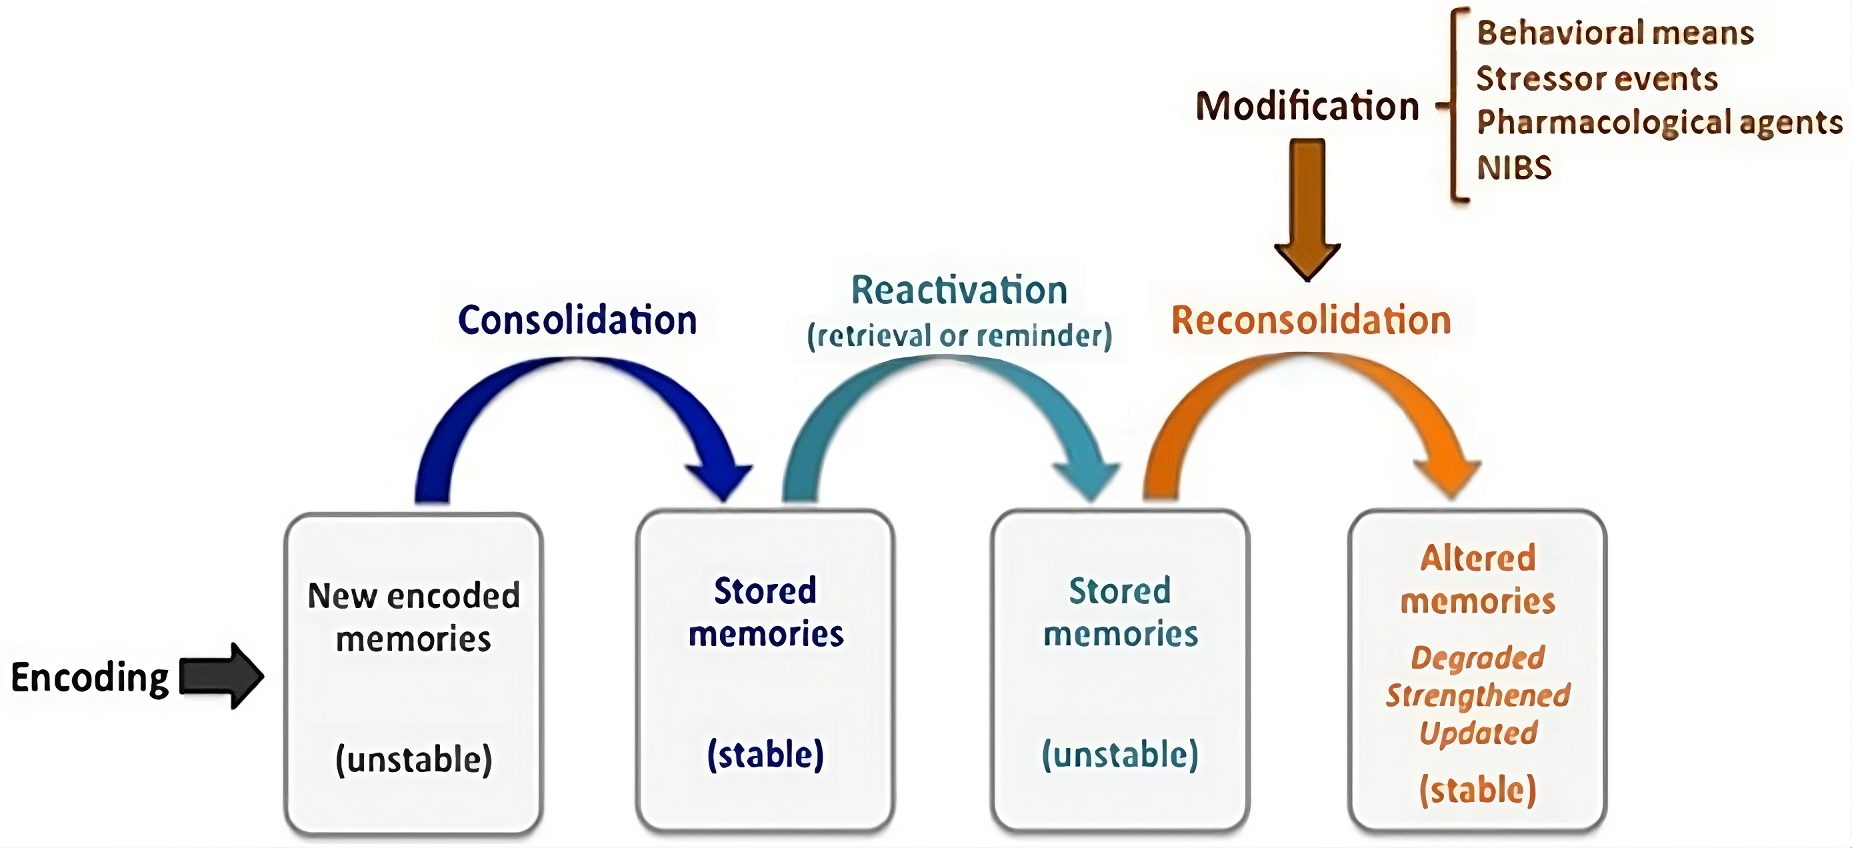
\includegraphics[width=0.7\linewidth]{./img/memory.png}
    \caption{Memory flow}
\end{figure}

\begin{remark}
    This mechanism is useful against traumatic memories.
\end{remark}

\begin{remark}
    The amygdala is responsible for storing conditioned responses while the hippocampus recognizes conditioned stimuli.

    Patients with a damaged amygdala only recognize \ac{cs} but do not act with any \ac{cr}.
    On the other hand, a damaged hippocampus results in patients that present a \ac{cr} without recognizing the \ac{cs}.
\end{remark}

\begin{example}[Reconsolidation disruption]
    Propranolol is a drug that disrupts amygdala-specific memory reconsolidation (i.e. the physiological response).
    A possible therapy to suppress a phobia is to trigger the fear memory and then administer propranolol to prevent its reconsolidation.
\end{example}



\section{Learning preconditions}

\subsection{Contiguity}
\marginnote{Contiguity}

Closeness between the \acl{cs} and the \acl{us}.

\begin{remark}
    The closer in time the stimuli are presented, the more likely the association will be created.
\end{remark}

Depending on when the \ac{cs} and \ac{us} are presented, conditioning can be:
\begin{descriptionlist}
    \item[Delay conditioning] \marginnote{Delay conditioning}
        The \ac{cs} is extended through the interstimulus interval (ISI) (i.e. time between the start of the \ac{cs} and the \ac{us}).

    \item[Trace conditioning] \marginnote{Trace conditioning}
        There is a delay (trace interval) between the \ac{cs} end and the \ac{us} start.

        Learning requires more trials and might be impossible if the trace interval is too long as the mental representation of the \ac{cs} decays.

    \begin{figure}[H]
        \centering
        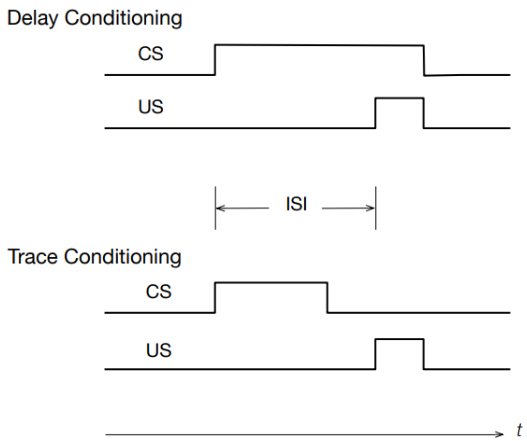
\includegraphics[width=0.45\linewidth]{./img/contiguity.png}
    \end{figure}
\end{descriptionlist}

\begin{example}
    Two groups of rats were exposed to a 6 seconds tone (\ac{cs}) followed by food delivery (\ac{us}) with a delay of: 
    \begin{itemize}
        \item 6 seconds (red).
        \item 18 seconds (purple).
    \end{itemize}

    \begin{figure}[H]
        \centering
        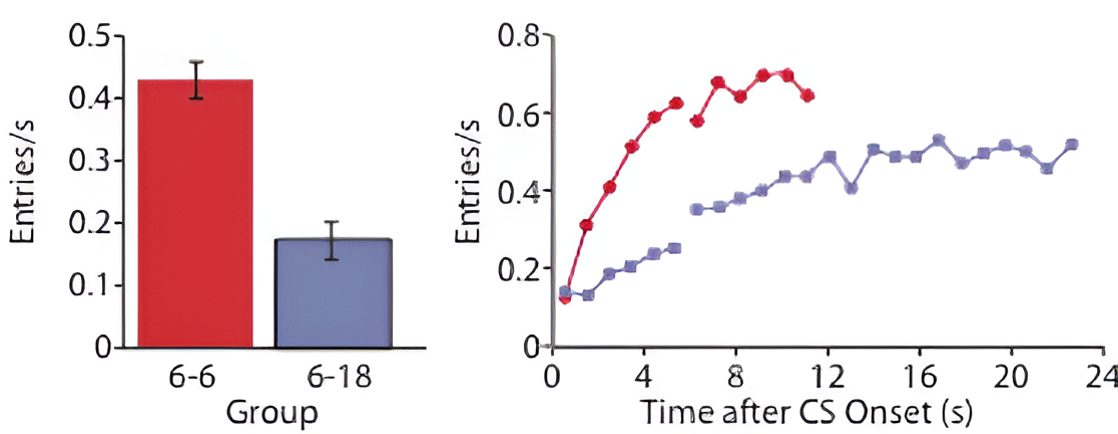
\includegraphics[width=0.55\linewidth]{./img/contiguity_rats.png}
        \caption{Number of entries (i.e. the rat checks the food tray) per second}
    \end{figure}
\end{example}


\subsection{Contingency}
\marginnote{Contingency}

Causal relationship between the \acl{cs} and the \acl{us}.

\begin{remark}
    Learning happens when:
    \[ \prob{\text{\ac{us} with \ac{cs}}} > \prob{\text{\ac{us} with no \ac{cs}}} \]
    In other words, the \ac{cs} should provide information regarding the \ac{us}.
\end{remark}

\begin{figure}[H]
    \centering
    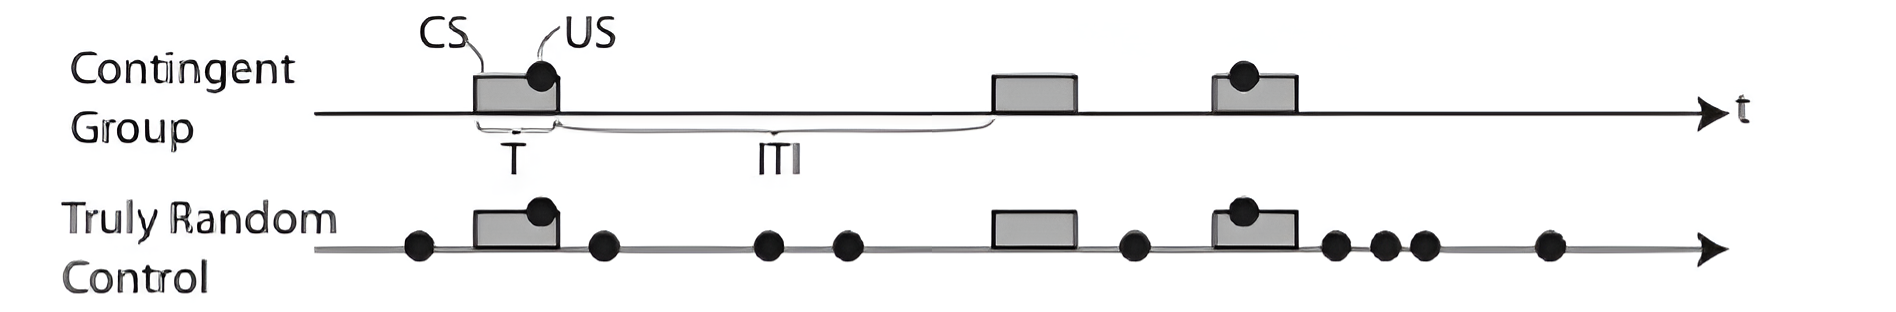
\includegraphics[width=0.6\linewidth]{./img/contingency.png}
    \caption{Example of contingent and random group}
\end{figure}

\begin{example}
    Two groups of rats are exposed to a shock paired with a bell ring.
    Contiguity is the same but contingency differs.

    Only the group where the shock is more likely with the bell learns the association.

    \begin{figure}[H]
        \centering
        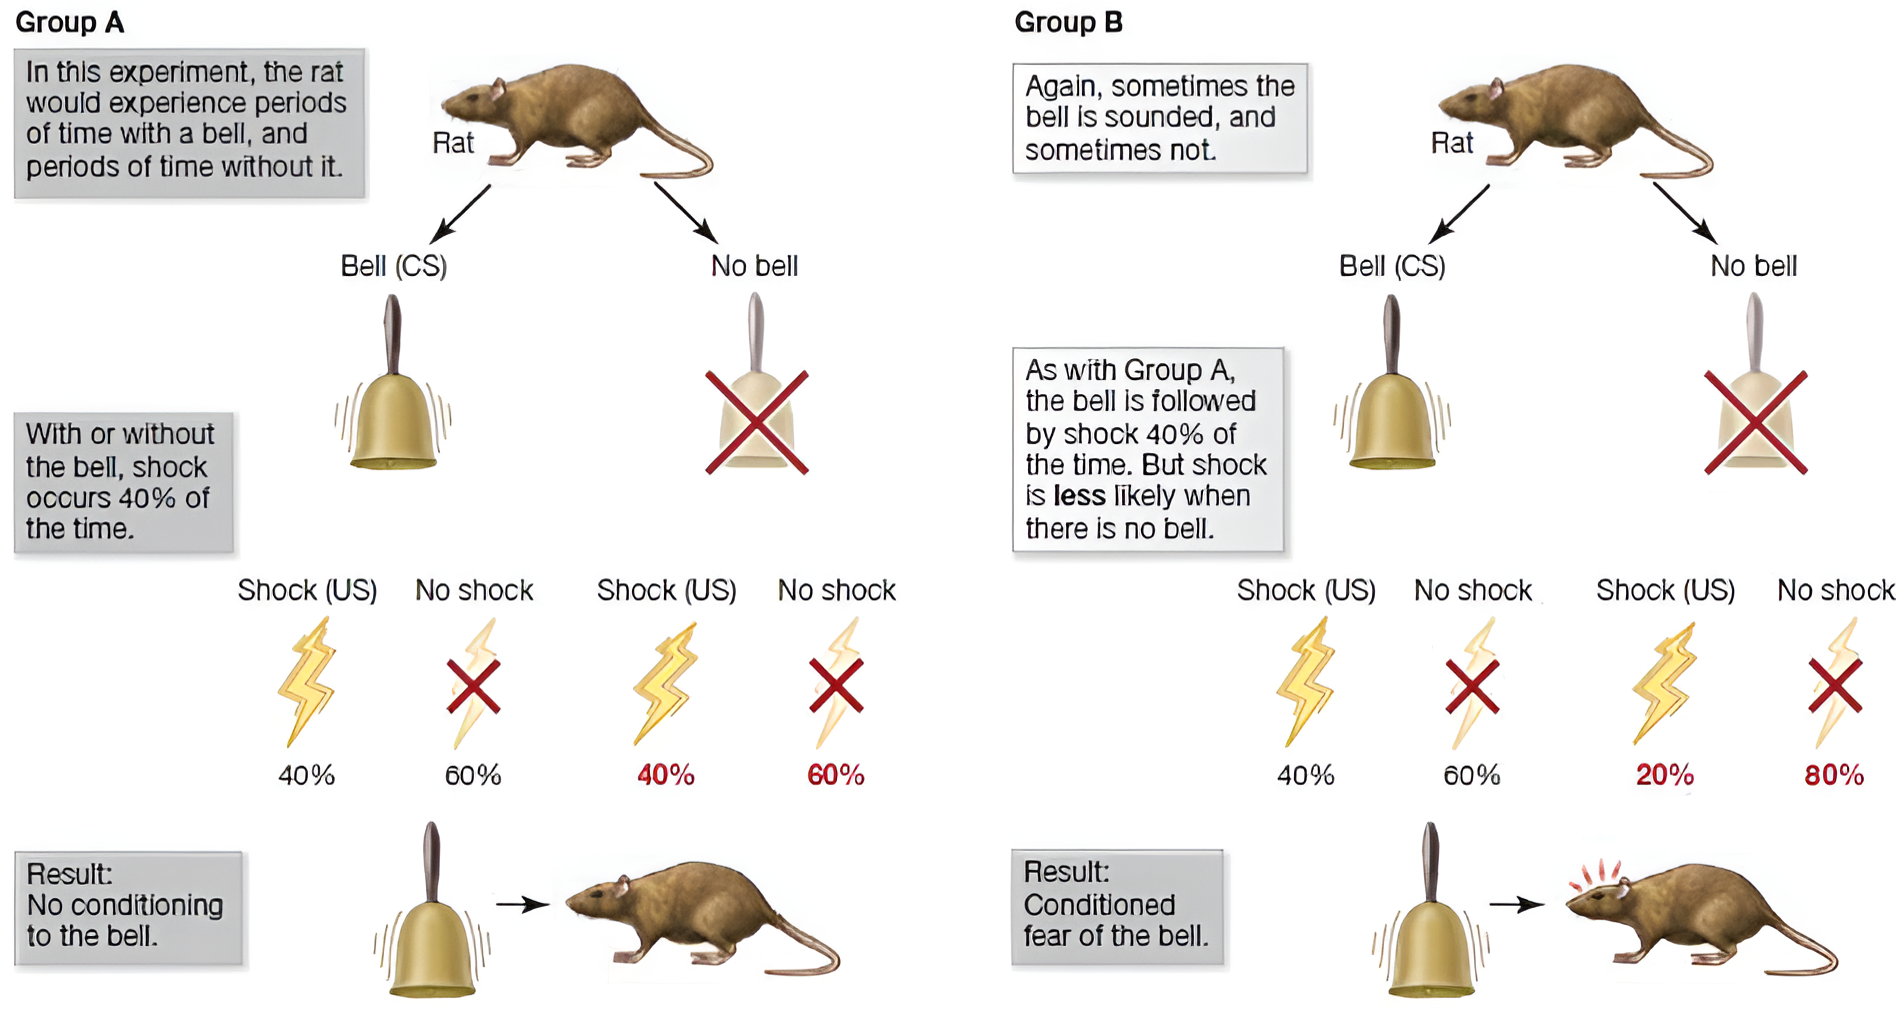
\includegraphics[width=0.8\linewidth]{./img/contingency_rats.png}
        \caption{Representation of the experiment}
    \end{figure}
\end{example}


\subsection{Surprise}

\begin{description}
    \item[Prediction error] \marginnote{Prediction error}
        Quantitative discrepancy between the expected and experienced outcome.
\end{description}

\begin{remark}
    Learning happens when the outcome is different from what was expected.
\end{remark}

\begin{figure}[H]
    \centering
    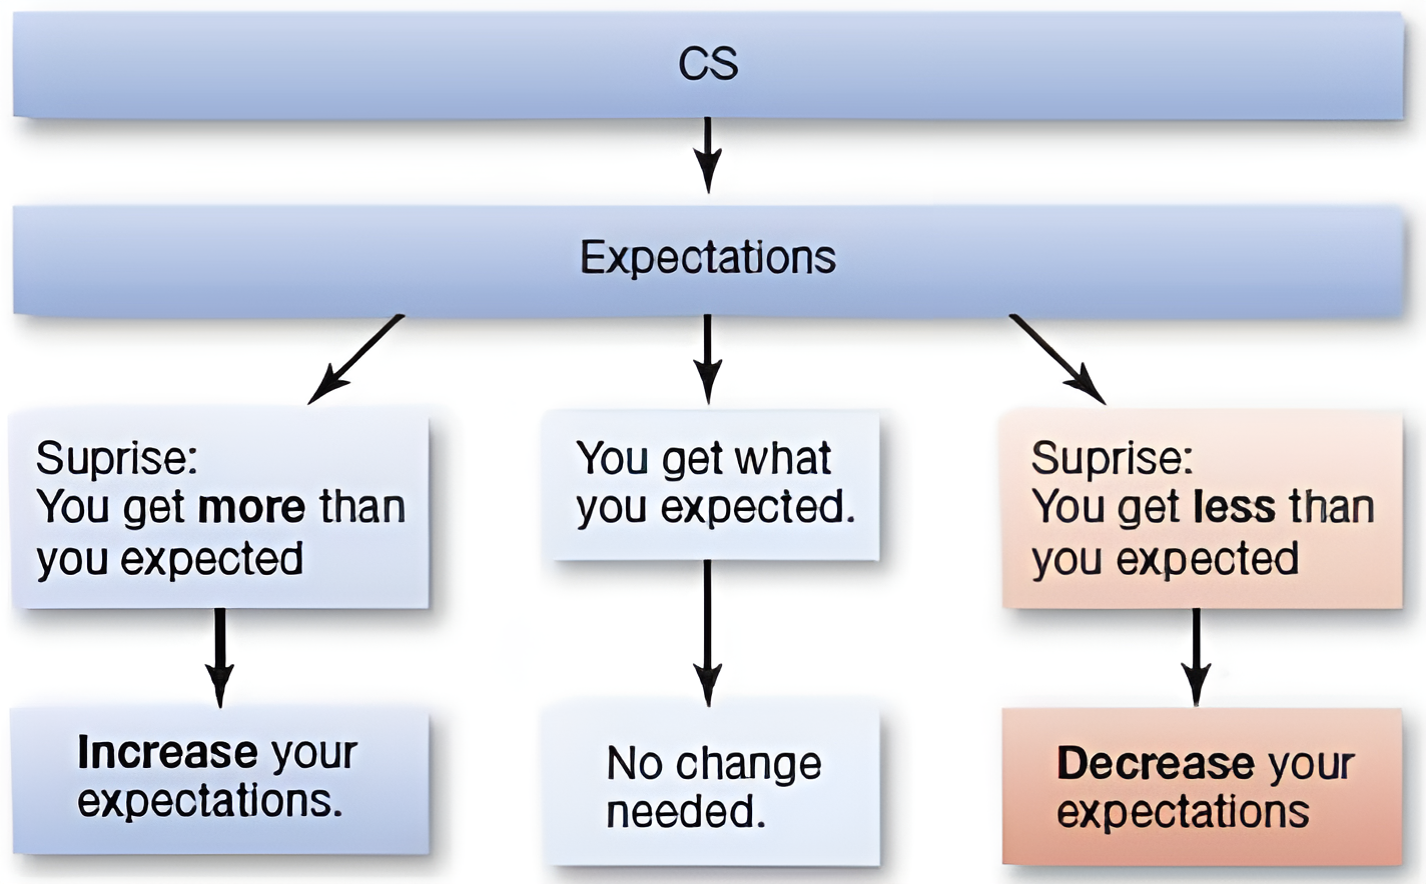
\includegraphics[width=0.4\linewidth]{./img/surprise.png}
    \caption{Learning outcome due to surprise}
\end{figure}

\begin{example}
    \phantom{}\\
    \begin{minipage}{0.65\linewidth}
        \begin{enumerate}
            \item A rat is taught that a hissing sound (\ac{cs}) is paired with a sexually receptive mate (\ac{us}).
            \item A light is added together with the hissing sound.
            \item When only the light is presented, the rat does not provide a response.
        \end{enumerate}

        The light is not learned as a \ac{cs} as it does not provide any new information on the \ac{us}.
    \end{minipage}
    \begin{minipage}{0.3\linewidth}
        \begin{figure}[H]
            \centering
            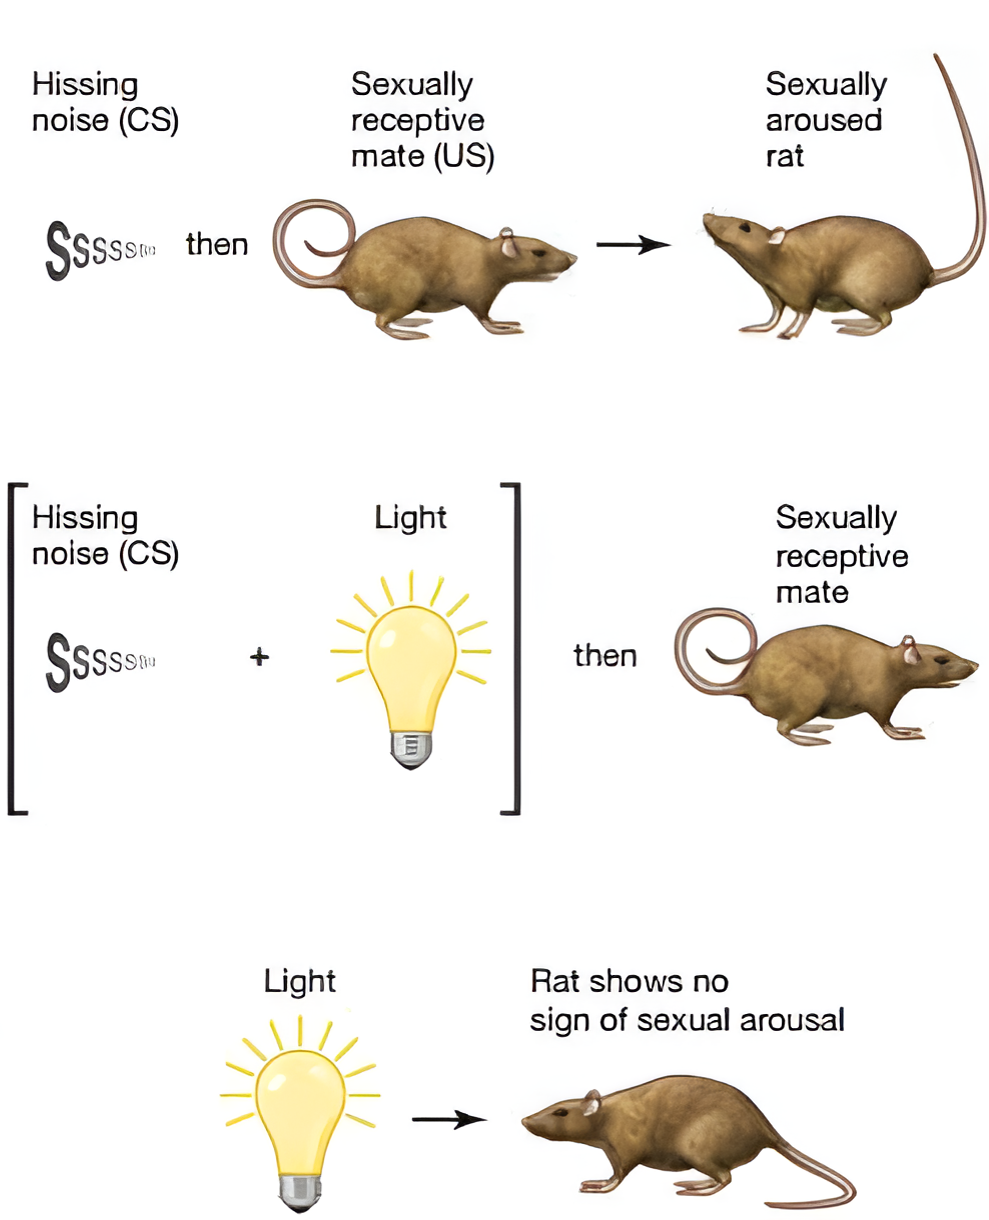
\includegraphics[width=\linewidth]{./img/surprise_rats.png}
        \end{figure}
    \end{minipage}
\end{example}